% The Why of Tali Forth
% Scot W. Stevenson

\section{The big picture}

This section provides background information on Forth, the 6502 processor, and
what anybody would want to combine the two. It can be safely skipped.

\subsection{The 6502 MPU}

Humanity reached the high point of processor design with the 6502\index{6502} in
1976. Created by a team including Chuck Peddle\index{Peddle, Chuck} and Bill
Mensch\index{Mensch, Bill}, it was the engine that powered the 8-bit home
computer revolution of the 1980s.\footnote{Rumor has it that there was another
MPU called `Z80'\index{Z80} at the same time, but it ended up being a mere
footnote.} The VIC-20\index{VIC-20}, Commodore PET\index{Commodore PET}, Apple
II\index{Apple II}, and Atari 800\index{Atari 800} all used the 6502, among
others. 

\begin{figure}[h !]
        \centering
        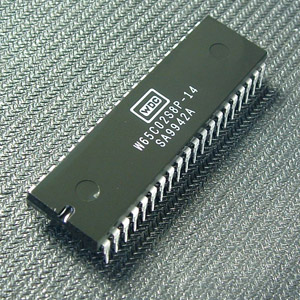
\includegraphics[width=0.5\textwidth]{pics/W65c02}
        \caption{\textit{The 65c02 MPU.} Photographer: Anthony King, released in 
        the public domain}
        \label{fig:65c02}
\end{figure}

More than 40 years later, the processor is still in production by the \href
{http://www.westerndesigncenter.com/wdc/w65c02s-chip.cfm} {Western Design
Center}\index{WDC}. Apart for commercial uses, there is an active hobbyist scene
centered on the website \href{http://6502.org/}{6502.org}.\index{6502.org} Quite
a number of people have built their own 8-bit computers based on this chip. 

The most important variant produced today is the \href
{https://en.wikipedia.org/wiki/WDC\_65C02}{65c02}\index{65c02}, a CMOS chip with
some additional instructions. Tali Forth 2 is specifically designed for this
chip and this chip only.

Why program in 8-bit assembler? The 65c02 is fun to work with because of its
clean instruction set architecture (ISA)\index{instruction
set!architecture}\index{ISA|see {instruction set}}. 


\subsection{Forth}

\begin{quote}
        But Forth is also like a high-wire act; if C gives you enough rope to
        hang yourself, Forth is a flamethrower crawling with cobras.
\end{quote}
\begin{flushright}
        -- Elliot Williams,\index{Williams, Elliot} \href{https://hackaday.com/2017/01/27/forth-the-hackers-language/}{
        \textit{Forth: The Hacker's Language}}
\end{flushright}

Forth\index{Forth|textbf} is black sheep among the program languages. Invented
by Chuck Moore\index{Moore, Chuck} in the 1960s for work with radio astronomy,
it is stack-based, uses reverse polish notation (RPN)\index{RPN|see {reverse
polish notation}}\index{reverse polish notation} and a threaded interpreter
model. 

(HIER HIER)

There is no way this document can support an introduction to Forth. There are
quite a number only, such as \textit{A Beginner's Guide to Forth} by
J.V.~Nobel\cite{nobel} or the classic (but slightly dated) \textit{Thinking in
Forth}\cite{brodie03} by Leo Brodie\index{Brodie, Leo}.  Gforth\index{Gforth}
comes with its own
\href{http://www.complang.tuwien.ac.at/forth/gforth/Docs-html/Tutorial.html}{tutorial}.

Once you have grasped the basic of the language, do yourself a favor and read
\textit{Thinking in Forth} by Brodie\cite{brodie84}\index{Brodie, Leo}. 


\section{Writing your own Forth}
